\documentclass[11pt,a4paper]{article}
\usepackage[utf8]{inputenc}
\usepackage[T1]{fontenc}
\usepackage{lmodern}
\usepackage[english]{babel}
\usepackage[a4paper,margin=2.4cm]{geometry}
\usepackage{amsmath,amssymb,mathtools}
\usepackage{graphicx}
\usepackage{booktabs}
\usepackage{multirow}
\usepackage{tabularx}
\usepackage{array}
\usepackage{enumitem}
\usepackage{xcolor}
\usepackage{tikz}
\usetikzlibrary{arrows.meta,positioning,calc,quantikz2}
\usepackage{pgfplots}
\pgfplotsset{compat=1.18}
\usepackage{caption}
\usepackage{subcaption}
\usepackage{microtype}
\usepackage{placeins}
\usepackage{float}
\usepackage[hidelinks]{hyperref}
\usepackage[nameinlink]{cleveref}
\ifdefined\bodyonlyflag
  \usepackage{comment}
  \excludecomment{figure}
  \excludecomment{figure*}
  \excludecomment{table}
\fi

\captionsetup{font=small,labelfont=bf}
\setlist{itemsep=0.15em,topsep=0.3em}
\newcolumntype{L}{>{\raggedright\arraybackslash}X}
\newcolumntype{P}[1]{>{\raggedright\arraybackslash}p{#1}}
\providecommand{\ket}[1]{\lvert #1\rangle}
\providecommand{\bra}[1]{\langle #1\rvert}
\DeclareMathOperator{\diag}{diag}

\begin{document}

\noindent
\begin{minipage}[c]{0.5\textwidth}
  
\includegraphics[height=2.0cm]{logos/CS.png}
\end{minipage}%
\hfill
\begin{minipage}[c]{0.45\textwidth}
  \raggedleft
  
\includegraphics[height=1.15cm]{logos/L2S_logo.png}
\end{minipage}

\vspace{0.8em}
\begin{center}
  {\LARGE\bfseries Quantum semantics and language models:\\[0.2em]
    from the semiotic square to trainable Hamiltonian predictors\par}
  \vspace{0.9em}
  {\large Ethan Bandasack \quad Malo Leroy \quad Thierry Zhang\par}
  \vspace{0.3em}
  {\small CentraleSupélec, Université Paris-Saclay \textperiodcentered{} Laboratoire des Signaux et Systèmes (L2S)\par
    Research track, case study 21 \textperiodcentered{} Supervisor: Zeno Toffano \textperiodcentered{} November 2026\par}
\end{center}

\begin{abstract}
  \noindent
  Quantum semantics describes meaning with Hilbert spaces, operators and measurement: the semiotic square of structural semantics can be written with Pauli operators, and compositional grammar shares its algebra with quantum circuits. Recent proposals go further and train quantum circuits as word models, but they are evaluated on very small corpora with permissive metrics. We surveyed this literature and then asked a narrower empirical question: does a trainable quantum component improve next-word prediction when it is compared with fair classical controls? We reimplemented the Quantum Context-Sensitive Embedding (QCSE) model in exact simulation, extended it into hybrid circuit models trained against scratch MLP and BERT references, and finally built direct predictors in which a learned Hamiltonian evolves a prepared state and the next token is read by the Born rule. The QCSE evaluation metric is satisfied by a constant bit prior, and the original model almost never recovers the exact word. In hybrid models the circuit contributes little: an identity circuit performs within a fraction of a point of trained ones, and a classical MLP leads on every endpoint. Hamiltonian learning works and coherent evolution beats a retrained dephased control, yet the best three-seed quantum model on WikiText-2 subwords still trails an equally exposed classical MLP, and its generated text is incoherent. No quantum advantage is demonstrated. We argue that the operator view of meaning remains a useful modelling language, and that a controlled test of semiotic constraints is the most direct next step.
\end{abstract}

\section{Introduction}

Statistical language models capture context well. How they represent relations between meanings, such as contradiction, antonymy or inclusion, is another matter: these relations stay implicit in their weights. Quantum semantics makes them explicit. Meanings become vectors in a Hilbert space, semantic relations become operators, and reading a text is modelled as a measurement~\cite{galofaro2018,dubois2026}. Compositional distributional semantics adds a principled way of combining word meanings according to grammar, with the same categorical structure as quantum processes~\cite{coecke2010}. Our subject asked how this formal rigour could be combined with the computational power of neural networks.

Trainable quantum circuits sit between these formal proposals and modern language models. QCSE~\cite{varmantchaonala2026} learns context-sensitive word representations directly from corpus statistics; other works translate Transformer blocks into circuits~\cite{liao2024,kong2025,khatri2024} or add quantum-inspired attention to small generative models~\cite{kuznetsov2026}. Their empirical support is thin. Corpora are small, runs are rarely repeated, and the classical baseline seldom receives the same input, target and budget.

We therefore asked a single question: \emph{does a trainable quantum component improve next-word prediction over fair classical controls?} We started from QCSE because it was the most concrete model of our reading list. Its metric turned out to reward label statistics, so we gave the circuit learned inputs and compared it with classical networks. When the circuit still contributed little, we removed the classical output layer altogether and let a learned Hamiltonian predict the next token by measurement. This report contributes:
\begin{enumerate}[label=(\roman*)]
  \item a short synthesis separating quantum-like semantics from trained quantum models (\cref{sec:background});
  \item an audit of QCSE, showing that its published metric does not measure word recovery;
  \item a hybrid benchmark against scratch MLP and BERT references, with left-only and bidirectional contexts;
  \item Hamiltonian predictors with Born-rule readout, developed step by step up to subword prediction on WikiText-2.
\end{enumerate}
All experiments are noiseless simulations. Methods and results follow in \cref{sec:methods,sec:results}, with discussion in \cref{sec:discussion}. Equations, extended results and configurations are in Appendices~\ref{app:math}, \ref{app:results} and~\ref{app:config}.

\section{Background}
\label{sec:background}

\paragraph{Quantum-like semantics.}
Galofaro, Toffano and Doan build word vectors from a Hyperspace Analogue to Language (HAL) co-occurrence matrix and read the relation between two words through Pauli observables~\cite{galofaro2018}. A correlation of $+1$ suggests that the words support each other in the text, $-1$ that they are opposed. The authors relate these operators to the semiotic square of Greimas, which organises a semantic category into contraries, contradictories and implications.

Dubois and Toffano make the correspondence explicit (\cref{fig:square}): $\sigma_z$ relates the contraries $S_1/S_2$, $\sigma_x$ the contradictories $S_1/\neg S_1$, and $\sigma_y$ the inclusion $S_1\to\neg S_2$. Eigenlogic then reads logical propositions as operators whose eigenvalues are truth values~\cite{dubois2026,toffano2020}. This vocabulary separates relations that a cosine similarity confuses, since antonyms often share contexts. What it does not yet provide is a rule mapping a text to a two-qubit state, or an evaluation on annotated relations.

\begin{figure}[!tb]
  \centering
  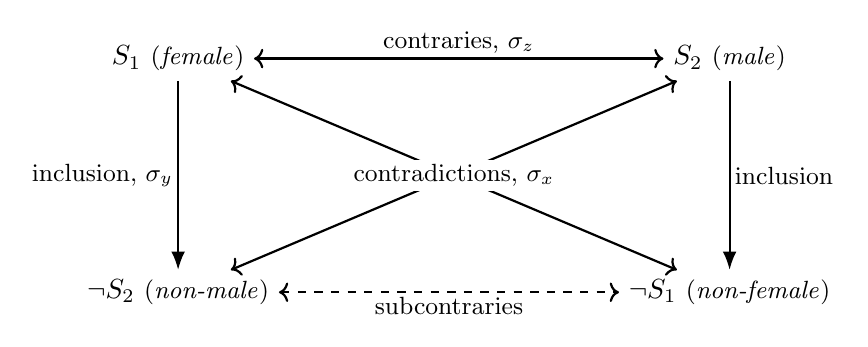
\begin{tikzpicture}[
      node distance=2.4cm and 5.2cm,
      term/.style={font=\normalsize},
      rel/.style={font=\small, fill=white, inner sep=1.5pt}]
    \node[term] (s1) {$S_1$ \small(\emph{female})};
    \node[term, right=of s1] (s2) {$S_2$ \small(\emph{male})};
    \node[term, below=of s1] (ns2) {$\neg S_2$ \small(\emph{non-male})};
    \node[term, below=of s2] (ns1) {$\neg S_1$ \small(\emph{non-female})};
    \draw[<->, thick] (s1) -- node[rel, above] {contraries, $\sigma_z$} (s2);
    \draw[<->, thick, dashed] (ns2) -- node[rel, below] {subcontraries} (ns1);
    \draw[<->, thick] (s1) -- (ns1);
    \draw[<->, thick] (s2) -- (ns2);
    \node[rel] at ($(s1)!0.5!(ns1)$) {contradictions, $\sigma_x$};
    \draw[-{Latex}, thick] (s1) -- node[rel, left] {inclusion, $\sigma_y$} (ns2);
    \draw[-{Latex}, thick] (s2) -- node[rel, right] {inclusion} (ns1);
  \end{tikzpicture}
  \caption{Semiotic square with the Pauli operators associated with each relation by Dubois and Toffano~\cite{dubois2026}, following Galofaro et al.~\cite{galofaro2018}. The example terms are theirs.}
  \label{fig:square}
\end{figure}

\paragraph{Compositional semantics.}
DisCoCat lifts the type reductions of a pregroup grammar to linear maps, so that the meaning of a sentence is a tensor contraction of word meanings and lives in a single sentence space~\cite{coecke2010}. Its diagrams compile into circuits, but the framework is not a generative language model.

\paragraph{Trainable quantum language models.}
\Cref{tab:related} summarises the models closest to our question. They range from a full circuit construction without experiments to small hybrids trained in simulation. None isolates what the quantum part adds over a classical model given the same information.

\begin{table}[!tb]
  \centering\small
  \caption{Trainable quantum language models related to this work.}
  \label{tab:related}
  \begin{tabularx}{\linewidth}{@{}lLL@{}}
    \toprule
    Work                                      & Quantum component                                                                 & Evidence reported                                                                                                                     \\
    \midrule
    QCSE~\cite{varmantchaonala2026}           & context-matrix angles, variational circuit, bit-wise readout of the centre word   & 110 English and 20 Fulani sentences; $85.8\%$ against $70.0\%$ for CBOW, a prediction counting as correct when half of its bits match \\
    GPT on a quantum computer~\cite{liao2024} & circuit construction of every block of a GPT decoder                              & theoretical; no training experiment                                                                                                   \\
    Quixer~\cite{khatri2024}                  & quantum Transformer built from linear combinations of unitaries                   & Penn Treebank; the classical Transformer reference scores better                                                                      \\
    HyQuT~\cite{kong2025}                     & variational circuits replacing selected linear layers of a generative Transformer & targeted replacements keep training stable, broad ones do not                                                                         \\
    QISA~\cite{kuznetsov2026}                 & quantum-inspired value transform in a GPT-1 style model                           & small embeddings, simulated; matches or improves classical attention on several metrics                                               \\
    \bottomrule
  \end{tabularx}
\end{table}

\section{Methods}
\label{sec:methods}

\paragraph{QCSE reimplementation.}
We implemented QCSE from its equations (\cref{fig:models}a, Appendix~\ref{app:qcse}). A window of $n$ context words gives an $n\times n$ matrix built from word indices and positional decay. Its entries are loaded as $R_X$ and $R_Z$ angles on $m=\lceil\log_2 V\rceil$ qubits, followed by a trainable $R_X/R_Z/\mathrm{CRZ}$ ansatz and Pauli-$Z$ measurement. Our simulator is exact and batched, and matches an independent Qiskit reference to within $10^{-15}$. We audited it on a miniature corpus before training it on our full corpus.

\begin{figure}[!tb]
  \centering
  \begin{subfigure}{\linewidth}
    \centering
    \begin{quantikz}[row sep=0.25cm, column sep=0.3cm]
      \lstick{$\ket{0}$} & \gate{H} & \gate[style={fill=blue!8}]{R_X(c)} & \gate[style={fill=blue!8}]{R_Z(c')} & \ctrl{1} & \qw & \gate[style={fill=orange!15}]{R_X(\theta)} & \gate[style={fill=orange!15}]{R_Z(\theta')} & \ctrl{1} & \qw & \meter{} \\
      \lstick{$\ket{0}$} & \gate{H} & \gate[style={fill=blue!8}]{R_X(c)} & \gate[style={fill=blue!8}]{R_Z(c')} & \targ{} & \ctrl{1} & \gate[style={fill=orange!15}]{R_X(\theta)} & \gate[style={fill=orange!15}]{R_Z(\theta')} & \gate{R_Z(\phi)} & \ctrl{1} & \meter{} \\
      \lstick{$\ket{0}$} & \gate{H} & \gate[style={fill=blue!8}]{R_X(c)} & \gate[style={fill=blue!8}]{R_Z(c')} & \qw & \targ{} & \gate[style={fill=orange!15}]{R_X(\theta)} & \gate[style={fill=orange!15}]{R_Z(\theta')} & \qw & \gate{R_Z(\phi')} & \meter{}
    \end{quantikz}
    \caption{QCSE: context-matrix angles $c$ (blue, repeated over encoding layers) and trainable ansatz angles $\theta,\phi$ (orange, repeated $M$ times); each qubit is measured in $Z$ and compared with one bit of the centre word.}
  \end{subfigure}

  \vspace{0.6em}
  \begin{subfigure}{\linewidth}
    \centering
    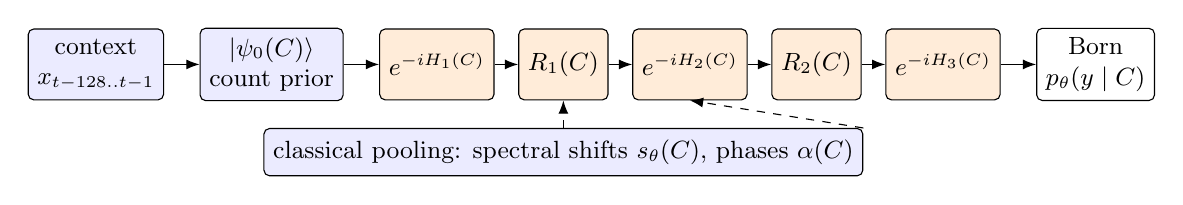
\begin{tikzpicture}[
      box/.style={draw, rounded corners=2pt, minimum height=0.9cm, align=center, font=\small},
      q/.style={box, fill=orange!15},
      c/.style={box, fill=blue!8},
      >={Latex}]
      \node[c] (ctx) {context\\$x_{t-128..t-1}$};
      \node[c, right=0.45cm of ctx] (prep) {$\ket{\psi_0(C)}$\\count prior};
      \node[q, right=0.45cm of prep] (h1) {$e^{-iH_1(C)}$};
      \node[q, right=0.3cm of h1] (r1) {$R_1(C)$};
      \node[q, right=0.3cm of r1] (h2) {$e^{-iH_2(C)}$};
      \node[q, right=0.3cm of h2] (r2) {$R_2(C)$};
      \node[q, right=0.3cm of r2] (h3) {$e^{-iH_3(C)}$};
      \node[box, right=0.45cm of h3] (m) {Born\\$p_\theta(y\mid C)$};
      \draw[->] (ctx) -- (prep);
      \draw[->] (prep) -- (h1);
      \draw[->] (h1) -- (r1);
      \draw[->] (r1) -- (h2);
      \draw[->] (h2) -- (r2);
      \draw[->] (r2) -- (h3);
      \draw[->] (h3) -- (m);
      \node[c, below=0.35cm of r1, minimum height=0.6cm] (pool) {classical pooling: spectral shifts $s_\theta(C)$, phases $\alpha(C)$};
      \draw[->, dashed] (pool.north) -- (r1.south);
      \draw[->, dashed] (pool.north east) -- (h2.south);
    \end{tikzpicture}
    \caption{Final Hamiltonian predictor on ten qubits: a count-based state is evolved by three context-dependent low-rank Hamiltonians interleaved with local phase rotations; the token register is measured directly, without a classical output layer.}
  \end{subfigure}
  \caption{The two quantum model families studied. Blue: classical inputs or computation; orange: trainable quantum operations.}
  \label{fig:models}
\end{figure}

\paragraph{Hybrid benchmark.}
The hybrid models replace the fixed encoding by a learned word embedding, mapped to rotation angles on eight qubits. A depth-two circuit follows, and a classical head reads local $X$, $Y$, $Z$ expectations to score every vocabulary word. We compared six circuit settings: CRZ, $ZZ$ and $XX$ chains, local rotations only, a frozen CRZ circuit, and the identity. The classical references were an MLP language model in the style of Bengio et al.~\cite{bengio2003} and a two-layer BERT~\cite{devlin2019}, both trained from scratch on the same word identifiers. Two tasks share the same targets: left-only prediction from four previous words (L4) and bidirectional prediction from two words on each side (L2R2).

\paragraph{Hamiltonian predictors.}
The last line of work has no classical head (\cref{fig:models}b, Appendix~\ref{app:ham}). The context prepares a state on the token register, a learned Hermitian operator $H$ evolves it, and the next token $y$ is drawn with probability $p_\theta(y\mid C)=|\bra{y}e^{-iH}\ket{\psi_C}|^2$. A dephased control, which removes all coherences before evolution, is retrained independently. Successive steps added low-rank evolution, an unmeasured auxiliary qubit, context-dependent phases and energies, a count-based initial state and classical context pooling. The final model has ten qubits (nine for the token, one auxiliary), three evolution stages of rank 128, and $1{,}073{,}900$ real parameters.

\paragraph{Data and protocol.}
Word-level studies used English sentence corpora, split by sentence group so that duplicated sentences never cross partitions. The final Hamiltonian studies used WikiText-2 raw articles~\cite{merity2016}, a 512-token byte-pair vocabulary fitted on training articles only, and 128 tokens of left context. Classical controls received the same inputs and update budgets, and checkpoints were selected on validation data only. \Cref{tab:metrics} lists the metrics. Hybrid and later Hamiltonian runs used 10\,GB slices of an NVIDIA A100, at most four at a time (Appendix~\ref{app:config}).

\begin{table}[!tb]
  \centering\small
  \caption{Metrics. NLL uses natural logarithms. $S$ is what one quantum measurement delivers; argmax requires the whole distribution.}
  \label{tab:metrics}
  \begin{tabularx}{\linewidth}{@{}llL@{}}
    \toprule
    Metric     & Definition                                                      & Used for                    \\
    \midrule
    NLL        & $-\frac1N\sum_t\log p_\theta(y_t\mid C_t)$, lower is better     & all word and subword models \\
    top-$k$    & target among the $k$ most probable words                        & hybrid benchmark ($k=1,5$)  \\
    $S$        & $\frac1N\sum_t p_\theta(y_t\mid C_t)$, success of one Born draw & Hamiltonian predictors      \\
    argmax     & top-1 accuracy of the full distribution                         & Hamiltonian predictors      \\
    half-bit   & at least half of the $m$ output bits match                      & QCSE, as published          \\
    exact word & all $m$ thresholded bits match                                  & QCSE audit and sweep        \\
    \bottomrule
  \end{tabularx}
\end{table}

\section{Results}
\label{sec:results}

\paragraph{The QCSE metric does not measure word recovery.}
Three findings came out of the audit (\cref{tab:summary}, Appendix~\ref{app:math}):
\begin{itemize}
  \item \emph{Metric.} For $m$ independent random bits, at least half match the target with probability $1/2$, and frequency-ranked identifiers make the bits unbalanced. On our miniature audit, a constant prior estimated from training targets scores $96.5\%$ on the half-bit criterion. QCSE after 50 epochs scores $56.1\%$ and recovers no word exactly. In a separate pilot, training on shuffled labels gave the same test loss as training on true labels.
  \item \emph{Inactive parameters.} The first encoding $R_X$ acts on an eigenstate, and the final diagonal ansatz gates cannot change $Z$ marginals. At least 19 of 58 ansatz parameters thus receive no gradient from the data term.
  \item \emph{Full scale.} With $V=10{,}864$ words on 14 qubits, the best of 44 configurations reaches $1.07\%$ exact-word test accuracy.
\end{itemize}

\begin{figure}[!tb]
  \centering
  \begin{subfigure}[t]{0.48\linewidth}
    \centering
    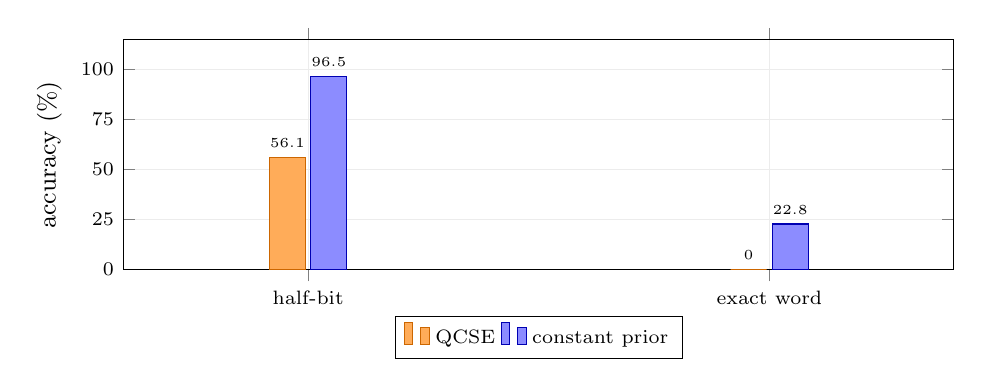
\begin{tikzpicture}
      \begin{axis}[
          width=\linewidth, height=4.5cm,
          ybar, bar width=13pt,
          ymin=0, ymax=115, ytick={0,25,50,75,100},
          ylabel={accuracy (\%)},
          symbolic x coords={half-bit,exact word}, xtick=data,
          enlarge x limits=0.4,
          tick label style={font=\scriptsize}, label style={font=\small},
          nodes near coords, every node near coord/.append style={font=\tiny},
          legend style={at={(0.5,-0.2)}, anchor=north, font=\scriptsize, legend columns=2},
          grid=major, grid style={gray!15}]
        \addplot[fill=orange!65, draw=orange!80!black] coordinates {(half-bit,56.1) (exact word,0)};
        \addplot[fill=blue!45, draw=blue!70!black] coordinates {(half-bit,96.5) (exact word,22.8)};
        \legend{QCSE,constant prior}
      \end{axis}
    \end{tikzpicture}
    \caption{QCSE audit: permissive scoring versus exact recovery (57 test targets).}
  \end{subfigure}\hfill
  \begin{subfigure}[t]{0.48\linewidth}
    \centering
    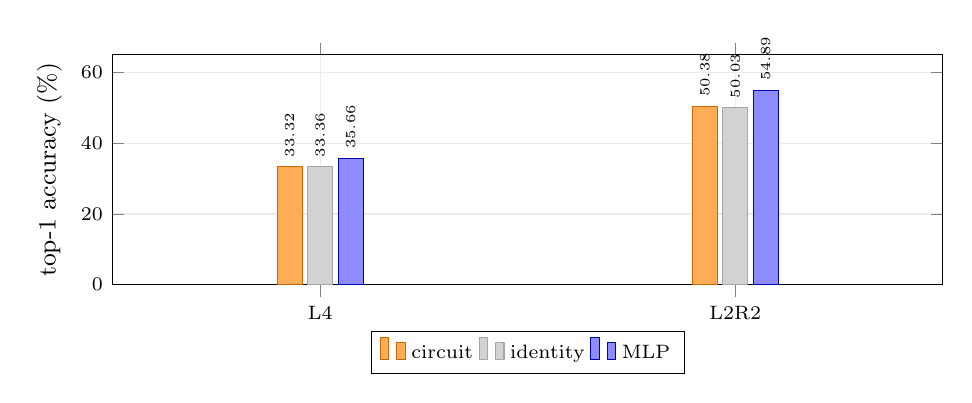
\begin{tikzpicture}
      \begin{axis}[
          width=\linewidth, height=4.5cm,
          ybar, bar width=9pt,
          ymin=0, ymax=65, ytick={0,20,40,60},
          ylabel={top-1 accuracy (\%)},
          symbolic x coords={L4,L2R2}, xtick=data,
          enlarge x limits=0.5,
          tick label style={font=\scriptsize}, label style={font=\small},
          nodes near coords, every node near coord/.append style={font=\tiny, rotate=90, anchor=west},
          legend style={at={(0.5,-0.2)}, anchor=north, font=\scriptsize, legend columns=3},
          grid=major, grid style={gray!15}]
        \addplot[fill=orange!65, draw=orange!80!black] coordinates {(L4,33.32) (L2R2,50.38)};
        \addplot[fill=gray!35, draw=gray!70] coordinates {(L4,33.36) (L2R2,50.03)};
        \addplot[fill=blue!45, draw=blue!70!black] coordinates {(L4,35.66) (L2R2,54.89)};
        \legend{circuit,identity,MLP}
      \end{axis}
    \end{tikzpicture}
    \caption{Circuits with classical output: two-seed validation means (252,120 targets).}
  \end{subfigure}

  \vspace{1em}
  \begin{subfigure}[t]{0.48\linewidth}
    \centering
    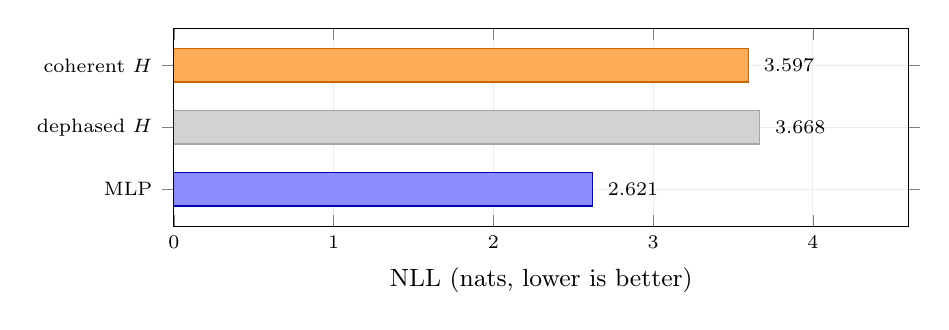
\begin{tikzpicture}
      \begin{axis}[
          width=0.9\linewidth, height=4.1cm,
          xbar, bar width=12pt, bar shift=0pt,
          xmin=0, xmax=4.6, xtick={0,1,2,3,4},
          xlabel={NLL (nats, lower is better)},
          ytick={1,2,3}, yticklabels={MLP,dephased $H$,coherent $H$},
          ymin=0.4, ymax=3.6,
          tick label style={font=\scriptsize}, label style={font=\small},
          nodes near coords, every node near coord/.append style={font=\scriptsize, anchor=west, xshift=2pt},
          point meta=explicit symbolic,
          grid=major, grid style={gray!15}]
        \addplot[fill=orange!65, draw=orange!80!black] coordinates {(3.597,3) [3.597]};
        \addplot[fill=gray!35, draw=gray!70] coordinates {(3.668,2) [3.668]};
        \addplot[fill=blue!45, draw=blue!70!black] coordinates {(2.621,1) [2.621]};
      \end{axis}
    \end{tikzpicture}
    \caption{Word-level Hamiltonian: three-seed test means (8,192 targets).}
  \end{subfigure}\hfill
  \begin{subfigure}[t]{0.48\linewidth}
    \centering
    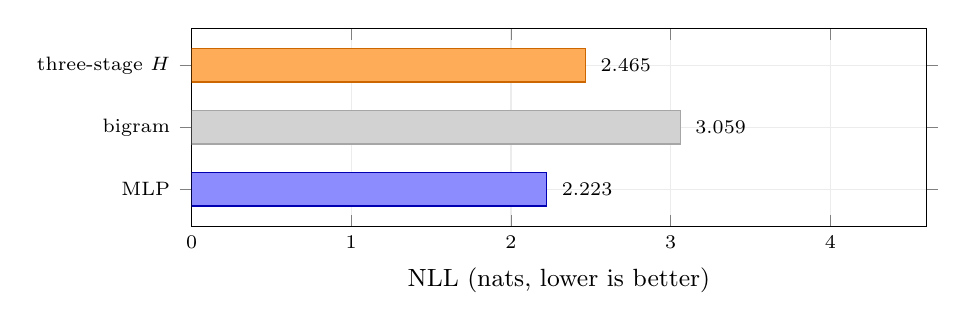
\begin{tikzpicture}
      \begin{axis}[
          width=0.9\linewidth, height=4.1cm,
          xbar, bar width=12pt, bar shift=0pt,
          xmin=0, xmax=4.6, xtick={0,1,2,3,4},
          xlabel={NLL (nats, lower is better)},
          ytick={1,2,3}, yticklabels={MLP,bigram,three-stage $H$},
          ymin=0.4, ymax=3.6,
          tick label style={font=\scriptsize}, label style={font=\small},
          nodes near coords, every node near coord/.append style={font=\scriptsize, anchor=west, xshift=2pt},
          point meta=explicit symbolic,
          grid=major, grid style={gray!15}]
        \addplot[fill=orange!65, draw=orange!80!black] coordinates {(2.465,3) [2.465]};
        \addplot[fill=gray!35, draw=gray!70] coordinates {(3.059,2) [3.059]};
        \addplot[fill=blue!45, draw=blue!70!black] coordinates {(2.223,1) [2.223]};
      \end{axis}
    \end{tikzpicture}
    \caption{WikiText-2 subwords: three-seed validation means (4,096 targets).}
  \end{subfigure}
  \caption{Main comparisons. Each panel uses a different task; compare models within a panel. In (b), circuit denotes CRZ for L4 and $ZZ$ for L2R2. The word and subword NLLs in (c,d) have different units of prediction. Detailed metrics appear in Appendix~\ref{app:results}.}
  \label{fig:summary}
\end{figure}

\paragraph{With a classical output layer, the circuit adds little.}
Across both tasks and both seeds, the MLP leads every reported metric (\cref{fig:summary}, Table~\ref{tab:robust}). Trained circuits stay within a few tenths of a percentage point of the identity. The $ZZ$ chain gains about $0.36$ top-5 points over identity in both tasks, but its left-only NLL and top-1 effects change sign between seeds. CRZ and $ZZ$ chains define the same function class after a change of angles, so their ranking cannot reflect a difference in expressivity.

Earlier cross-validation and held-out checks support this result (Table~\ref{tab:campaigns}). Over five folds and three seeds, a trained circuit beat identity by $0.23$ top-1 points at $2.7$ times the simulator cost, with gains in some folds and losses in others. On a held-out left-only test with three seeds, the two stayed within $0.05$ top-1 points while the MLP led by about two.

Could optimisation itself be the obstacle? In 9,216 initial-gradient evaluations, gradients shrink with register size but stay clearly nonzero up to twelve qubits: we found no evidence of a barren plateau~\cite{mcclean2018,cerezo2021}, although trained states and larger registers were not probed.

\paragraph{Hamiltonian learning works.}
On Tatoeba, with 256 words and four context words, training a full Hermitian matrix lowers test NLL from $6.59$ to $3.60$. The coherent model beats its retrained dephased control on NLL and one-draw success. On two toy tasks coherence is decisive: $100\%$ against $8.33\%$ on modular composition.

\paragraph{But it does not catch up with classical models.}
On WikiText-2 subwords, retained steps lowered quantum validation NLL from $4.28$ to $2.47$ for the three-seed reference. The MLP's total reduction was larger (\cref{fig:progress}). At the replicated endpoint, one-draw success is $28.52\%$ versus $39.45\%$ for the MLP, and argmax accuracy $44.10\%$ versus $50.35\%$; the NLL gap is $0.24$ nats. The quantum model beats bigram counts, but its saved continuations remain incoherent. Sequential token loading, streamed context blocks and Hamiltonian factor normalisation did not improve on their controls (Table~\ref{tab:rejected}).

\begin{figure}[!tb]
  \centering
  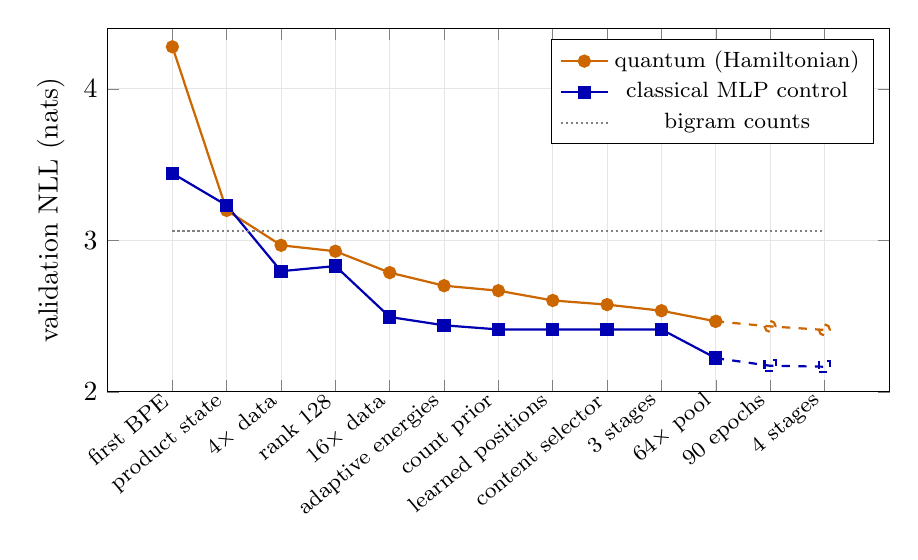
\begin{tikzpicture}
    \begin{axis}[
        width=0.95\linewidth, height=6.2cm,
        ylabel={validation NLL (nats)},
        xtick={1,...,13},
        xticklabels={first BPE, product state, $4\times$ data, rank 128, $16\times$ data, adaptive energies, count prior, learned positions, content selector, 3 stages, $64\times$ pool, 90 epochs, 4 stages},
        xticklabel style={rotate=40, anchor=east, font=\footnotesize},
        ymin=2.0, ymax=4.4,
        grid=major, grid style={gray!20},
        legend style={at={(0.98,0.97)}, anchor=north east, font=\footnotesize},
        mark size=2pt]
      \addplot[thick, color=orange!80!black, mark=*] coordinates {
          (1,4.2773) (2,3.1975) (3,2.9673) (4,2.9281) (5,2.7870) (6,2.7007)
          (7,2.66776) (8,2.60325) (9,2.57588) (10,2.53554) (11,2.46546)};
      \addlegendentry{quantum (Hamiltonian)}
      \addplot[thick, color=blue!70!black, mark=square*] coordinates {
          (1,3.4424) (2,3.2306) (3,2.7966) (4,2.8303) (5,2.4941) (6,2.4393)
          (7,2.41207) (8,2.41207) (9,2.41207) (10,2.41207) (11,2.22277)};
      \addlegendentry{classical MLP control}
      \addplot[thick, dashed, color=orange!80!black, mark=o, forget plot] coordinates {
          (11,2.46546) (12,2.43218) (13,2.40905)};
      \addplot[thick, dashed, color=blue!70!black, mark=square, forget plot] coordinates {
          (11,2.22277) (12,2.17231) (13,2.16622)};
      \addplot[gray, densely dotted, thick, domain=1:13] {3.0593};
      \addlegendentry{bigram counts}
    \end{axis}
  \end{tikzpicture}
  \caption{Retained design steps of the Hamiltonian predictor on WikiText-2 subwords (512 tokens, 128-token context). Each point is the step's quantum model and its strongest equally exposed MLP control; steps 7 to 11 are three-seed means, steps 12 and 13 (dashed) single seeds. Steps change data or recipe, so only vertical gaps are like-for-like comparisons.}
  \label{fig:progress}
\end{figure}

\section{Discussion and conclusion}
\label{sec:discussion}

Most of our gains came from classical ingredients. Learned embeddings, count-based initial states, context pooling and broader training coverage each helped the quantum models more than any change of circuit family or depth, and they helped the classical controls even more. The one quantum-specific effect we could isolate is a coherence benefit over a restricted dephased model, which is not an advantage over a competent classical predictor. The QCSE audit also shows why a control must share the target and the metric: a half-bit criterion rewards label statistics, not language understanding.

These conclusions have limits. Everything ran in noiseless simulation, so we say nothing of hardware trainability or speed, and we did not cost state preparation or the compilation of a learned Hamiltonian into gates. The WikiText comparisons reuse one validation set; we deliberately left its test split unscored. Most comparisons rest on two or three seeds, some quantum and classical models differ in parameter count, and stronger classical models such as small Transformers were not tuned to the same extent.

We did not test the semiotic square experimentally. The most direct continuation is a relation-classification task. A two-qubit Pauli bottleneck would be trained with differentiable constraints derived from the square (symmetric contraries, inverted inclusion, involutive negation), and compared with the same constraints on a classical head. That experiment would test the semantic hypothesis of quantum relations directly, which next-word prediction could not.

In short, quantum language models are trainable in simulation, and coherence can matter within a restricted model family. In our experiments, however, every quantum or hybrid model was matched or outperformed by a classical model given the same information.

\FloatBarrier
\section*{Acknowledgements}
We thank Zeno Toffano for proposing and supervising this subject. Experiments ran on a DGX A100 server. Large language model assistants were used for literature search, code and drafting; all numbers were checked against the experiment records.

\bibliographystyle{unsrt}
\ifdefined\bodyonlyflag\else
  \bibliography{references}
\fi

\ifdefined\bodyonlyflag\else
  \clearpage
  \appendix

  \section{Mathematical details}
  \label{app:math}

  \subsection{QCSE encoding and readout}
  \label{app:qcse}
  For a window of $n$ context words with dictionary indices $\mathrm{idx}_i$ and $V$ vocabulary words, let $\vartheta_i=2\pi\,\mathrm{idx}_i/V$. The main QCSE context matrix is
  \begin{equation}
    C_{ij}=e^{-\alpha|i-j|}\sin(\omega\vartheta_i)\cos(\omega\vartheta_j)+\vartheta_i ,
  \end{equation}
  where $i,j$ are positions in the window. Its $n^2$ entries are read row by row, zero-padded, and split into
  \begin{equation}
    L=\left\lceil \frac{n^2}{2m}\right\rceil \ \text{encoding layers of $2m$ angles},\qquad m=\lceil\log_2 V\rceil ,
  \end{equation}
  two angles per qubit. After an initial Hadamard on each qubit, every layer applies $R_X$ then $R_Z$ to each qubit and a chain of adjacent CNOTs. The ansatz repeats $M$ times trainable $R_X$, $R_Z$ and a CRZ chain. The output is the vector of marginals
  \begin{equation}
    P(b_q=1)=\tfrac12\bigl(1-\langle Z_q\rangle\bigr),\qquad q=1,\dots,m,
  \end{equation}
  trained with binary cross-entropy against the bits of the centre word.

  The matrix depends on arbitrary dictionary indices, so relabelling the vocabulary changes the input. It is a numerical feature map, not a semantic Hamiltonian.

  \paragraph{Inactive gates.}
  Since $\ket{+}$ is an eigenstate of $X$, $R_X(a)\ket{+}=e^{-ia/2}\ket{+}$: the first-layer $R_X$ angles only add a global phase. For any diagonal unitary $D$, $D^\dagger Z_q D=Z_q$, so the final $R_Z$ and CRZ block of the ansatz cannot change any $Z$ marginal. For $m=10$ and $M=2$ this leaves at least 19 of the 58 ansatz angles without data gradient.

  \paragraph{Chance level of the half-bit criterion.}
  If the $m$ predicted bits are independent and uniform, the probability that at least $\lceil m/2\rceil$ of them match is
  \begin{equation}
    2^{-7}\textstyle\sum_{k=4}^{7}\binom{7}{k}=\tfrac{64}{128}=\tfrac12,\qquad 2^{-5}\sum_{k=3}^{5}\binom{5}{k}=\tfrac{16}{32}=\tfrac12,
  \end{equation}
  whereas the exact word is recovered with probability $2^{-m}$. With frequency-ranked identifiers the high-order bits of frequent words are mostly zero, which a constant prior exploits.

  For even $m$, the criterion includes the tie, giving chance success $\tfrac12+2^{-m-1}\binom{m}{m/2}$ rather than $1/2$.

  \paragraph{Marginals are not the Born distribution.}
  Scoring a valid word $w$ with binary code $b(w)$ from independent marginals $p_q$ gives
  \begin{equation}
    \log P(w)=\mathrm{const}+\textstyle\sum_q b_q(w)\log\frac{p_q}{1-p_q},
  \end{equation}
  a fixed linear head on the log-odds. Different joint states share the same marginals, so this readout discards correlations that the joint Born distribution would use.

  \subsection{Circuit equivalences}
  With $R_P(a)=e^{-iaP/2}$, a controlled phase satisfies
  \begin{equation}
    \mathrm{CRZ}_{ct}(g)=R_{Z,t}(g/2)\,R_{ZZ,ct}(-g/2).
  \end{equation}
  When each layer also contains free local $R_Z$ angles, the map from CRZ to $ZZ$ parameters is invertible, so both chains define the same set of unitaries; only their initialisation and optimisation coordinates differ. With a product input and one two-qubit gate crossing each cut per layer, the Schmidt rank across any cut is at most $2^{\text{depth}}$, which makes depth-two chains efficiently simulable by matrix product states.

  \subsection{Hamiltonian predictors}
  \label{app:ham}
  \paragraph{First model.}
  With $W$ previous words, fixed amplitudes $\tilde\psi_j(C)=\sum_{a=0}^{W-1}\sqrt{0.7^a}\,i^a\,\mathbf 1[w_{t-1-a}=j]$ are normalised to $\psi_C$, and
  \begin{equation}
    p_\theta(y\mid C)=\bigl|(e^{-iH_\theta}\psi_C)_y\bigr|^2,\qquad H_\theta=H_\theta^\dagger .
  \end{equation}
  All $d^2$ real coordinates of $H$ are trained. The dephased control replaces $\psi\psi^\dagger$ by its diagonal before evolution:
  \begin{equation}
    p_{\text{coh}}(y)=\Bigl|\textstyle\sum_j U_{yj}\psi_j\Bigr|^2,\qquad
    p_{\text{deph}}(y)=\textstyle\sum_j |U_{yj}|^2|\psi_j|^2 .
  \end{equation}

  \paragraph{Final model.}
  Tokens are byte-pair identifiers, $V=512$, so nine qubits hold the token and one auxiliary qubit is added ($D=1024$). The initial state is built from smoothed training bigram counts:
  \begin{equation}
    \ket{\psi_0(C)}=\sum_{y}\sqrt{q(y\mid x_{t-1})}\,\ket{y}\ket{0},\qquad
    q(y\mid x)=\frac{n_{xy}+10\,\hat p(y)}{\sum_z n_{xz}+10},
  \end{equation}
  where $n_{xy}$ counts training transitions and $\hat p$ is the training unigram distribution. Each stage $\ell$ has a rank-128 Hamiltonian with context-dependent energies,
  \begin{equation}
    H_\ell(C)=Q_\ell\diag\bigl(e_\ell+s_\theta(C)\bigr)Q_\ell^\dagger,\qquad Q_\ell\in\mathbb C^{1024\times128},\ Q_\ell^\dagger Q_\ell=I,
  \end{equation}
  and local phases $R_\ell(C)=\bigotimes_{k=1}^{10}R_Z(\alpha_{\ell k}(C))$ separate the stages:
  \begin{equation}
    p_\theta(y\mid C)=\sum_{a\in\{0,1\}}\bigl|\bra{y,a}e^{-iH_3(C)}R_2(C)e^{-iH_2(C)}R_1(C)e^{-iH_1(C)}\ket{\psi_0(C)}\bigr|^2 .
  \end{equation}
  The shifts $s_\theta(C)$ and angles $\alpha(C)$ come from a classical pooling of the context with learned position weights and a 16-dimensional query/key selector. Zero energies reproduce the bigram baseline exactly.

  \paragraph{One draw versus argmax.}
  $S$ is the success rate of one measurement. It differs from argmax accuracy, which a single shot cannot deliver, and from $e^{-\mathrm{NLL}}$, which is a geometric mean.

  \section{Extended results}
  \label{app:results}

  \subsection{QCSE}

  \begin{table}[H]
    \centering\small
    \caption{QCSE audit on a miniature corpus (window 4, ten qubits, two ansatz layers, 177 training and 57 test targets from disjoint sentence groups, 50 epochs at learning rate $3\times10^{-4}$).}
    \label{tab:audit}
    \begin{tabular}{@{}lrrrr@{}}
      \toprule
      Model                        & Test BCE & Bit acc. (\%) & Exact word (\%) & Half-bit (\%) \\
      \midrule
      QCSE, initial                & 0.7283   & 47.4          & 0.0             & 54.4          \\
      QCSE, epoch 50               & 0.7200   & 47.9          & 0.0             & 56.1          \\
      constant training bit prior  & 0.5029   & 74.7          & 22.8            & 96.5          \\
      mean of context bits         & 2.6731   & 64.4          & 0.0             & 93.0          \\
      linear model on context bits & 0.4964   & 73.5          & 15.8            & 94.7          \\
      \bottomrule
    \end{tabular}
  \end{table}

  \begin{table}[H]
    \centering\small
    \caption{Other QCSE studies.}
    \label{tab:qcse-other}
    \begin{tabularx}{\linewidth}{@{}P{0.42\linewidth}L@{}}
      \toprule
      Study                                                                                          & Outcome                                                                                                                            \\
      \midrule
      Ordering pilot: 19 configurations $\times$ 3 seeds, 729-word alphabetical vocabulary, window 8 & word indices, layer order and gate order mostly change the initial state; no quantum run recovers an exact word                    \\
      Shuffled training labels, same pilot                                                           & test BCE $0.7203\pm0.0101$ against $0.7214\pm0.0095$ with true labels                                                              \\
      Pretrained Qwen embeddings, linear head                                                        & 8 of 57 test words recovered exactly                                                                                               \\
      Full-corpus sweep: 44 configurations of learning rate, $\alpha$, window, depth and batch size  & best: $\alpha=1$, learning rate $3\times10^{-4}$, window 2, 64 layers; $1.121\%$ validation and $1.068\%$ test exact-word accuracy \\
      \bottomrule
    \end{tabularx}
  \end{table}

  \subsection{Learned encoders, attention and circuits with classical output layers}

  \begin{table}[H]
    \centering\small
    \caption{Learned-encoder prototypes on capped phrase corpora (cosine retrieval of the target word).}
    \label{tab:semantic}
    \begin{tabularx}{\linewidth}{@{}P{0.42\linewidth}L@{}}
      \toprule
      Comparison                                           & Outcome                                                                   \\
      \midrule
      Learned embeddings, small circuit, classical decoder & $14.7\%$ cosine top-1 with a trained or a frozen circuit                  \\
      Same, combined-source corpus                         & $17.4\%$ without circuit against $16.8\%$ with a trained circuit          \\
      One quantum attention layer against no circuit       & test cross-entropy $4.6504\to4.6084$, but cosine top-1 $15.04\%\to9.94\%$ \\
      Learned against fixed QCSE inputs                    & learned inputs clearly better in every setting                            \\
      \bottomrule
    \end{tabularx}
  \end{table}

  \begin{table}[H]
    \centering\small
    \caption{Exploratory DGX A100 campaigns before the final circuit benchmark (10\,GB slices, at most four concurrent jobs). Corpus of 202,172 sentences, $V=10{,}864$.}
    \label{tab:campaigns}
    \begin{tabularx}{\linewidth}{@{}P{0.2\linewidth}P{0.27\linewidth}L@{}}
      \toprule
      Campaign                            & Design                                                                                 & Main lesson                                                                                                                                                               \\
      \midrule
      Timed cross-validation, 90 fits     & 6 models $\times$ 5 folds $\times$ 3 seeds; up to $50\times5{,}000$ draws              & trained circuit $+0.23$ top-1 points over identity at $2.7\times$ the cost, fold averages of both signs; QCSE ($7.89\%$) below the training-frequency baseline ($7.96\%$) \\
      Screen, 156 records                 & 52 arms $\times$ 3 folds; $100\times20{,}000$ draws                                    & identity as accurate as the trained circuit; deeper QCSE costs more without gain                                                                                          \\
      Follow-up, 258 fits and 30 refits   & learning-rate selection, then 5 folds $\times$ 3 seeds and held-out refits, both tasks & MLP-32 beats BERT-32 in every paired fit; held-out left-only top-1 $33.43\%$ (CRZ) against $33.47\%$ (identity), for 132 against 7.4 median minutes per fit               \\
      Gradient probes, 288 conditions     & 2 to 12 qubits, depths 2 and 8, two initialisation scales                              & initial gradients shrink with size but stay clearly nonzero                                                                                                               \\
      Target and causal controls, 40 fits & 8 models $\times$ 2 seeds $\times$ 2 tasks, common targets                             & final comparison, Table~\ref{tab:robust}                                                                                                                                  \\
      \bottomrule
    \end{tabularx}
  \end{table}

  \begin{table}[H]
    \centering\small
    \caption{Final comparison of circuits with a classical output layer, means over seeds 47 and 48 on the same 252,120 validation targets. Accuracies in \%.}
    \label{tab:robust}
    \begin{tabular}{@{}lrrrrrrr@{}}
      \toprule
                    &         & \multicolumn{3}{c}{Left-only (L4)} & \multicolumn{3}{c}{Bidirectional (L2R2)}                                                                      \\
      \cmidrule(lr){3-5}\cmidrule(l){6-8}
      Model         & Params  & NLL                                & top-1                                    & top-5          & NLL             & top-1          & top-5          \\
      \midrule
      MLP-32        & 368,880 & \textbf{3.2487}                    & \textbf{35.66}                           & \textbf{61.46} & \textbf{2.2064} & \textbf{54.89} & \textbf{77.45} \\
      BERT-32       & 385,394 & 3.3304                             & 34.08                                    & 59.55          & 2.3080          & 51.72          & 75.55          \\
      q8 CRZ        & 186,190 & 3.4664                             & 33.32                                    & 58.12          & 2.4684          & 50.23          & 73.60          \\
      q8 identity   & 186,144 & 3.4708                             & 33.36                                    & 57.94          & 2.4779          & 50.03          & 73.53          \\
      q8 local      &         & 3.4711                             & 33.19                                    & 57.95          & 2.4811          & 49.99          & 73.45          \\
      q8 frozen CRZ &         & 3.4744                             & 33.52                                    & 57.90          & 2.4699          & 50.10          & 73.63          \\
      q8 $XX$       &         & 3.4655                             & 33.38                                    & 58.12          & 2.4853          & 50.04          & 73.48          \\
      q8 $ZZ$       &         & 3.4685                             & 33.26                                    & 58.30          & 2.4572          & 50.38          & 73.87          \\
      \bottomrule
    \end{tabular}
  \end{table}

  \paragraph{Paired effects.}
  With 10,000 paired seed and sentence bootstrap draws (nominal $95\%$, uncorrected):
  \begin{itemize}
    \item $ZZ-$identity top-5 is $+0.36$ points $[+0.24,+0.50]$ left-only and $+0.35$ points $[-0.01,+0.69]$ bidirectional;
    \item left-only CRZ against frozen CRZ improves NLL by $0.008$ and top-5 by $0.22$ points but lowers top-1 by $0.20$ points, with the same signs in both seeds.
  \end{itemize}

  \subsection{Hamiltonian predictors}

  \begin{table}[H]
    \centering\small
    \caption{Hamiltonian learning on word and toy tasks (test sets; means over three confirmation seeds for Tatoeba, five seeds for toy tasks).}
    \label{tab:tatoeba}
    \begin{tabular}{@{}llrrr@{}}
      \toprule
      Task                                             & Model                  & NLL    & $S$ (\%) & Argmax (\%) \\
      \midrule
      \multirow{6}{*}{\shortstack[l]{Tatoeba, 256 words,                                                          \\4 context words, 8 qubits}}
                                                       & initial coherent $H$   & 6.5861 & 1.91     & 2.57        \\
                                                       & trained coherent $H$   & 3.5974 & 6.76     & 24.21       \\
                                                       & retrained dephased $H$ & 3.6683 & 5.71     & 19.51       \\
                                                       & MLP, 64,852 parameters & 2.6205 & 24.77    & 38.29       \\
                                                       & all-training bigram    & 2.6877 & 19.90    & 34.46       \\
                                                       & unigram                & 4.2408 & 4.55     & 16.98       \\
      \midrule
      \multirow{2}{*}{modular composition, 16 symbols} & coherent $H$           &        &          & 100.00      \\
                                                       & dephased $H$           &        &          & 8.33        \\
      \multirow{3}{*}{handwritten digits, 6 qubits}    & coherent $H$           &        &          & 91.96       \\
                                                       & dephased $H$           &        &          & 61.88       \\
                                                       & MLP                    &        &          & 95.43       \\
      \bottomrule
    \end{tabular}
  \end{table}

  \begin{table}[H]
    \centering\small
    \caption{Ideas rejected by their controls (validation NLL; reference in brackets).}
    \label{tab:rejected}
    \begin{tabular}{@{}P{0.42\linewidth}P{0.52\linewidth}@{}}
      \toprule
      Idea                                            & Outcome                                                    \\
      \midrule
      quantum walk on a co-occurrence graph           & NLL 4.296 against 3.462 for classical directed propagation \\
      coherent separation of recent and older context & 3.566 against 3.488 with the coherence removed             \\
      sequential token-ordered loading                & 3.117 [product state 2.967], 3.4 h per fit                 \\
      learned measurement basis                       & 2.92786 [2.92811], no useful change                        \\
      training directly for one-draw success          & $S$ 34.36\% but NLL 8.10 and repetitive text               \\
      streaming context blocks through Hamiltonians   & 3.298 [pooled 2.973]                                       \\
      cosine learning-rate decay                      & 2.7013 [constant 2.7021]                                   \\
      older-context dropout                           & 2.529 [2.540], interval includes zero                      \\
      fourth stage rather than wider stages           & 2.40905 [width-matched 2.41051], interval includes zero    \\
      normalised Hamiltonian factors                  & 2.664 [2.432]                                              \\
      \bottomrule
    \end{tabular}
  \end{table}

  \paragraph{Context length and generation.}
  With the expanded training pool, the full 128-token context beat a retrained 16-token model on NLL ($-0.012$, interval $[-0.020,-0.005]$) but not on one-draw success or argmax. A 64-token continuation sampled from the seed-22 model for the prompt ``The history of'' begins: \emph{``its first game ream , butvarBan7 was an untrHMNmanedthe Pecr8 Germania , New Ingaglas an delfirst there is''}.

  \section{Experimental configurations}
  \label{app:config}

  \begin{table}[H]
    \centering\small
    \caption{Data of each study. Splits are by sentence or article group; numbers count prediction targets.}
    \label{tab:config-data}
    \begin{tabularx}{\linewidth}{@{}lP{0.17\linewidth}lllL@{}}
      \toprule
      Study            & Corpus                     & Context      & Vocabulary & Qubits  & Train / validation / test               \\
      \midrule
      QCSE audit       & 1,000 phrases              & 4 words      & corpus     & 10      & 177 / -- / 57                           \\
      QCSE sweep       & phrases, cleaned sentences & 2 to 8 words & 10,864     & 14      & grouped split                           \\
      Hybrid campaigns & 202,172 sentences          & L4, L2R2     & 10,864     & 4 to 14 & 3 or 5 folds, 20\% outer test           \\
      Final hybrid     & 202,172 sentences          & L4, L2R2     & 10,864     & 8       & 1,014,085 / 252,120 / unused            \\
      Tatoeba $H$      & 246,072 sentences          & 4 words      & 255 + UNK  & 8       & 32,768 / 4,096 / 8,192                  \\
      WikiText-2 $H$   & raw articles               & 128 tokens   & 512 BPE    & 10      & pool 2,097,152 / 4,096 / 8,192 unscored \\
      \bottomrule
    \end{tabularx}
  \end{table}

  \begin{table}[H]
    \centering\small
    \caption{Training of each study. Draws are sampled with replacement unless stated; A100 slices have 10\,GB.}
    \label{tab:config-train}
    \begin{tabularx}{\linewidth}{@{}lLLll@{}}
      \toprule
      Study            & Budget                                                                        & Optimiser                                                & Seeds           & Hardware    \\
      \midrule
      QCSE audit       & 50 epochs                                                                     & Adam on SPSA gradients, lr $3\times10^{-4}$, BCE with L2 & 11              & CPU         \\
      QCSE sweep       & 10 sampled epochs                                                             & lr $3\times10^{-4}$ to $10^{-3}$, batch 16 to 256        & --              & A100        \\
      Hybrid campaigns & $50\times5{,}000$ to $100\times20{,}000$ draws                                & Adam, learning-rate grid                                 & 1 to 3 per fold & A100 slices \\
      Final hybrid     & $100\times20{,}000$ draws, batch 64                                           & Adam, lr 0.003                                           & 47, 48          & A100 slice  \\
      Tatoeba $H$      & 30 epochs, batch 512, clipping 5, float64                                     & Adam, lr 0.001 ($H$), 0.003 (MLP)                        & 61 to 63        & CPU         \\
      WikiText-2 $H$   & 30 epochs of 524,288 positions without replacement; 30,720 updates, batch 512 & Adam, lr 0.003; MLP cosine decay to 0.0003               & 11, 22, 33      & A100 slice  \\
      \bottomrule
    \end{tabularx}
  \end{table}

  Model sizes: final Hamiltonian model 1,073,900 real parameters, its MLP control 750,460; hybrid models in Table~\ref{tab:robust}. Hamiltonian checkpoints are selected on validation NLL; the final hybrid comparison scores the last epoch.
\fi

\end{document}
